\documentclass{beamer}
\newcommand{\name}{Claus }
\usetheme{Berlin}
\usecolortheme{beaver}
\usepackage[german]{babel}
\usepackage{graphicx}
\usepackage{xcolor}
\begin{document}
\title{NSD Skills Projekt}
\author{Kai Renken}
\date{\today}

\frame{\titlepage}
\setcounter{tocdepth}{1}

\frame{\frametitle{Ablauf}\tableofcontents}

\section{Was ist das Skills-Projekt?} 
\frame{\frametitle{Was ist das Skills-Projekt?}
	\begin{itemize}
		\pause
		\item Wir bauen eine Anwendung zur Organisation der Fähigkeiten (Skills) von Mitarbeitern bei neusta
		\pause
		\item Es gibt einen Katalog mit verfügbaren Skills inklusive einer Gewichtung (Relevanz für das Unternehmen)
		\pause
		\item Es gibt ein Portal, um meine Skills zu erfassen \\ (Wie gut kann ich was?)
		\pause
		\item Ich kann Erfolge sammeln (Stichwort "Gamification")
		\pause
		\item Über meine Skills und Erfolge kann ich einem Profil zugeordnet werden (Junior, Professional, Senior)
		\pause
		\item Das aktuelle Profil kann Grundlage transparenterer Gehaltsverhandlungen sein (Stichwort: "Gehaltsbänder")
	\end{itemize}
}
\section{Wie funktioniert das genau?}
\frame{\frametitle{Wie funktioniert das genau?}
	\begin{itemize}
		\pause
		\item Ich bin \name und möchte mehr Geld verdienen!
		\pause
		\item Meine \textcolor{blue}{Rolle} ist Java-Entwickler.
		\pause
		\item Bin ich \textcolor{red}{Junior}, \textcolor{red}{Professional} oder \textcolor{red}{Senior}?
	\end{itemize}
}
\subsection{Welches Profil habe ich?}
\frame{\frametitle{Welches Profil habe ich?}
	\begin{itemize}
		\pause
		\item 
	\end{itemize}
	\pause
}

\section{Technischer Rahmen}
\subsection{Architektur / Tech-Stack}
	\frame{\frametitle{Architektur / Tech-Stack?}
		\begin{itemize}
			\pause
			\item Kotlin
			\pause
			\item Maven
			\pause
			\item Spring Boot
			\pause
			\item PostgreSQL
			\pause
			\item Hexagonale Architektur
			\pause
			\item Domain Driven Design
			\pause
			\item Microsoft Azure AD
		\end{itemize}
		\pause
}
\subsection{Inner Source}
\subsection{Domänenmodell}
	\frame{\frametitle{Domänenmodell}
		\centering
		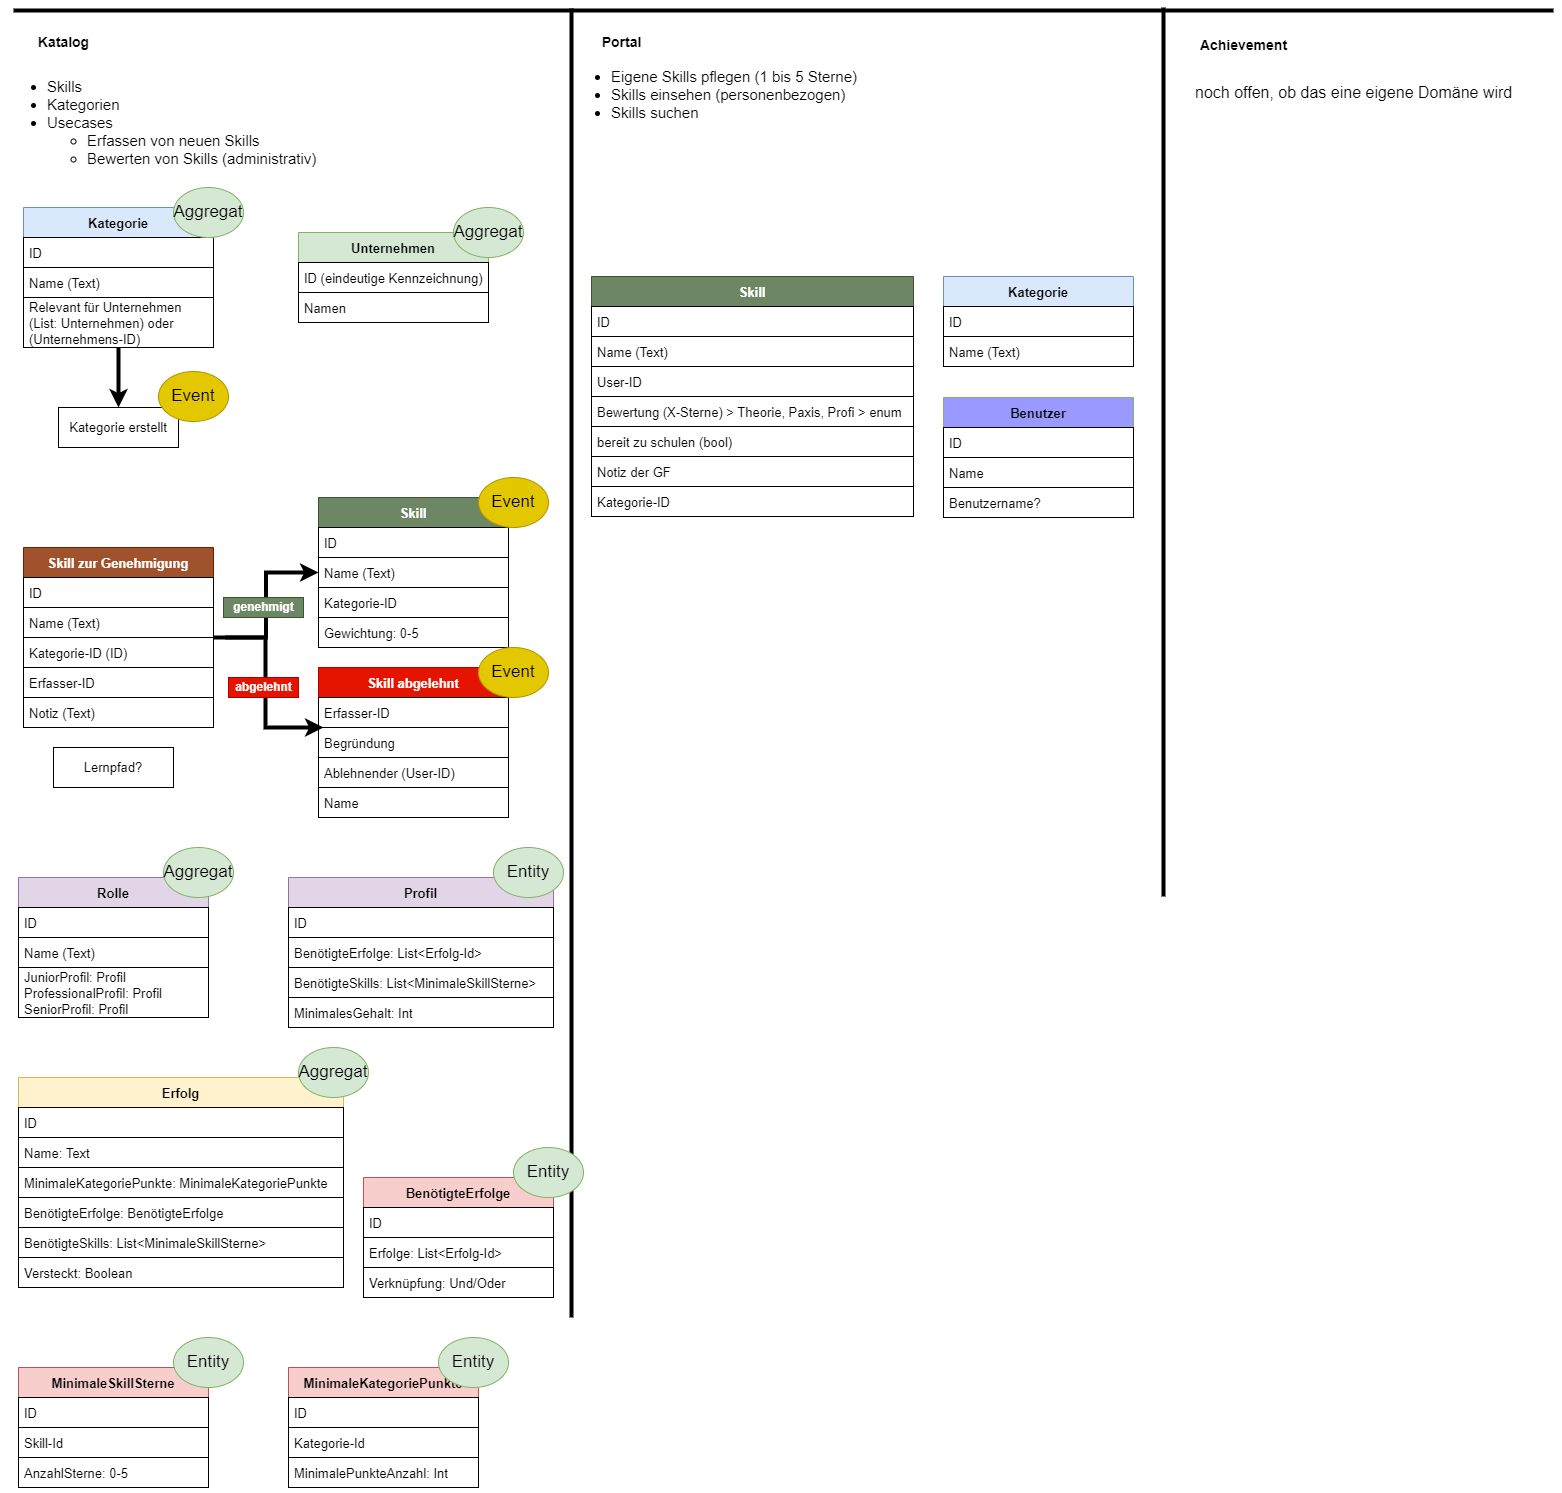
\includegraphics[scale=0.1]{domain_model.png}
}
\end{document}